% CAPITULO 3-------------------------------------------------------------------

\chapter{TAREFA 3: DESENVOLVIMENTO WEB}
\label{sec:tarefa3}

A palavra \textit{web} pertence ao vocabulário da língua inglesa e significa “rede”. Mesmo pertencendo ao léxico inglês o termo é amplamente utilizado em português como muitos outros com a mesma origem. Este conceito é utilizado dentro do espaço da tecnologia para referir-se a um sistema de interligação de documentos e recursos de forma geral, através da internet. O termo tanto pode se referir a uma página de internet, a um lugar virtual (\textit{website}) ou a um servidor. Este documento eletrônico contem informações adaptadas ao espaço em que se encontram de forma que possam ser acessadas por usuários do mundo todo que utilizam um determinado navegador.

Hoje em dia este acesso pode se dar a partir de um computador ou de qualquer outro dispositivo móvel. Uma página web é o nome que se da a um documento eletrônico. Web é a forma resumida e adaptada de \textbf{WWW} ( \textit{World Wide Web}). A estas páginas se podem ter acesso através de uma conexão de internet e estão compostas por textos, informações, links e aplicações informáticas. As páginas \textit{web} normalmente funcionam como uma espécie de cartão de apresentação digital. Empresas, pessoas particulares ou organizações, usam este recurso para apresentar suas idéias ou para fornecer informações. As páginas web geralmente se encontram em formato HTML, que é a linguagem utilizada nelas e que permite operar com links, etc.

Por meio delas se pode acessar outras páginas, “navegando” entre \textit{links}. Uma \textit{website} ( palavra feita da união dos termos ingleses web+site) é o lugar onde de reunem várias páginas webs dentro de um mesmo domínio e relacionadas entre si. O servidor web, por outro lado, é o computador ou a unidade onde se executam determinados software. Ou seja, é um programa utilizado para transferir páginas web. A \textit{world wide web} (web) tem sua origem (embora apenas a idéia à principio) em 1980 com o desenvolvimento de um projeto usado para armazenar informações associadas entre elas.

O projeto se denominava ENQUIRE e foi desenvolvido pelo inglês Tim Bernes-Lee. A idéia foi sendo melhorada ao longo dos anos e em 1991 foi publicado oficialmente o primeiro \textit{website}, mas só em 1994 foi dado o grande impulso á comercialização da \textit{web}. Hoje em dia a WWW é um espaço que pode ser acessado de forma globalizadas onde as pessoas podem formar, informar ou informar-se através de dispositivos conectados a Internet. \cite{web}

\section{A Importância da \textit{WEB}}

Para muitos, a grande conquista do milênio foi o surgimento da Rede Mundial de
Computadores. Durante duas décadas a Internet ficou restrita ao ambiente acadêmico e científico e
só em 1987 que pela primeira vez, foi liberado o seu uso comercial nos EUA. Mas só 5 anos depois,
em 1992, que a rede virou "moda". Começaram a aparecer, nos EUA, várias empresas provedoras
de acesso e no ano seguinte já era comum em universidades, estudantes criarem suas "páginas" com
informações pessoais.

No Brasil, a primeira espinha dorsal conectada à internet eram alguns centros de pesquisas
e universidades, além de algumas organizações não governamentais. Em 1994 começaram a
funcionar os primeiros serviços web do Brasil e começou a ser testado o acesso discado com fins
comerciais. No ano seguinte foi liberado o uso comercial da internet no Brasil e a partir de recursos
à disposição dos usuários como facilidade de acesso, o surgimento de provedores e portais de
serviços, possibilitaram um aumento considerável de usuários.

A internet passou a ser utilizada por vários segmentos sociais. Os estudantes passaram a
buscar informações para pesquisas escolares, enquanto jovens utilizavam para pura diversão e
entretenimento. As salas de chat tornaram-se pontos de encontro para um bate papo virtual a
qualquer instante, desempregados iniciavam buscas de emprego por meio de sites de agências de
emprego ou enviando currículos por \textit{e-mail} e então as empresas, de médio e grande porte,
entenderam que a Internet era um excelente caminho para melhorar seus lucros e resultados.

A internet revolucionou o “mundo dos negócios”, sendo uma ferramenta estratégica vital
para as empresas dos mais variados setores. A cultura empresarial mudou drasticamente, com a
comunicação em tempo real através da internet as organizações passaram a responder rápido as
novas tendências do mercado, além de encontrar e conquistar seu publico alvo com relativa
eficiência. Isso se da através da imensa gama de informação que se pode conseguir na rede, ou mais
especificamente nas redes sociais, é possível identificar grupos étnicos tendências, preferências,
opiniões e muito mais, além de levantar dados de qualquer relevância para qual quer negócio que
atue no setor comercial. \cite{evolucao}

\section{Funcionamento do Acesso Web}

A \textit{Internet} é uma rede que interconecta computadores e outros dispositivos como o seu celular em escala global para a transferência de dados entre eles. Já a \textit{World Wide Web} é uma aplicação onde páginas são interligadas através de links e que se utiliza da \textit{Internet} para funcionar.

Antes de abordar sobre a Web, precisamos conhecer um pouco sobre rede de computadores. Uma rede de computadores é a interconexão entre computadores que permite a comunicação de dados entre si. Esta comunicação pode ser feita através de cabos ou sem fios.

\begin{figure}[H]
    \centering
    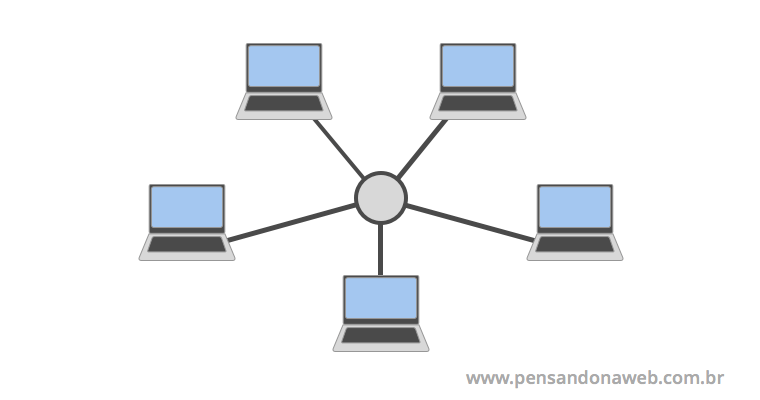
\includegraphics[width=0.7\linewidth]{dados/figuras/rede}
    \caption{Rede de computadores}
    \label{fig:rede}
\end{figure}

Partindo do principio que iremos acessar o site da Empresa T-Shirt, devemos abrir o navegador \textit{internet} de preferência e na barra de endereço digitar: www.tshirt.com.br passados alguns segundos a página inicial da empresa é exibida.

O acesso ao \textit{site} da empresa, só foi possível, pois os computadores possuem um endereço numérico único chamado endereço IP. Para que o acesso à página desejada, seja realmente realizado, o computador do cliente, precisa antes estabelecer uma conexão com o computador onde a página solicitada está hospedada.

Para simplificar, iremos chamar \textbf{cliente}, o computador utilizado para acesso ao site e \textbf{servidor}, o computador aonde a página esta hospedada.

\begin{figure}[H]
    \centering
    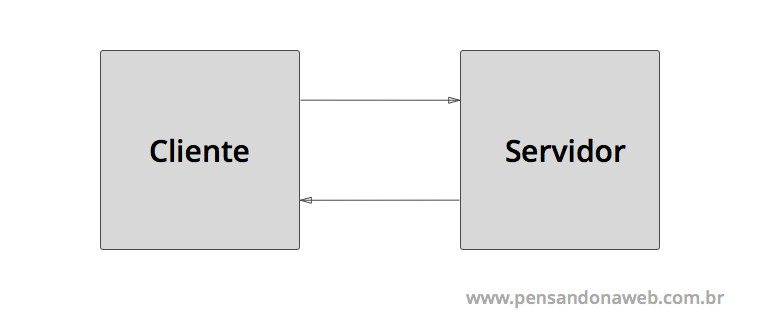
\includegraphics[width=0.7\linewidth]{dados/figuras/clientserver}
    \caption{Diagrama cliente x servidor}
    \label{fig:clientserver}
\end{figure}

Uma vez conhecido o endereço IP do destino a qual deseja se conectar, o cliente precisa estabelecer uma conexão com o servidor.

Este tipo de conexão utiliza o protocolo TCP ou \textit{Transmission Control Protocol} e é através deste protocolo que o cliente e o servidor conversam entre si. Através desta conexão ocorre o envio de pacotes, fragmentos menores dos dados que serão trafegados que contém informações como a porta de origem, a porta de destino e a sequência que devem ser reconstruídos ao chegar no destino.

O que acontece quando a conexão é estabelecida? Existe uma aplicação conhecida como servidor web que recebe e manipula todos os pacotes recebidos.

o HTTP ou \textit{Hypertext Transfer Protocol} e é o idioma que os navegadores e os servidores web conversam. É por meio deste idioma que o seu navegador informa ao servidor \textit{web} qual a sua versão, qual o seu idioma, se aceita conteúdo compactado ou não e qual página foi solicitada. Da mesma forma, é através deste idioma que o servidor web informa ao seu navegador se a página solicitada existe, qual o seu formato.

\begin{figure}[H]
    \centering
    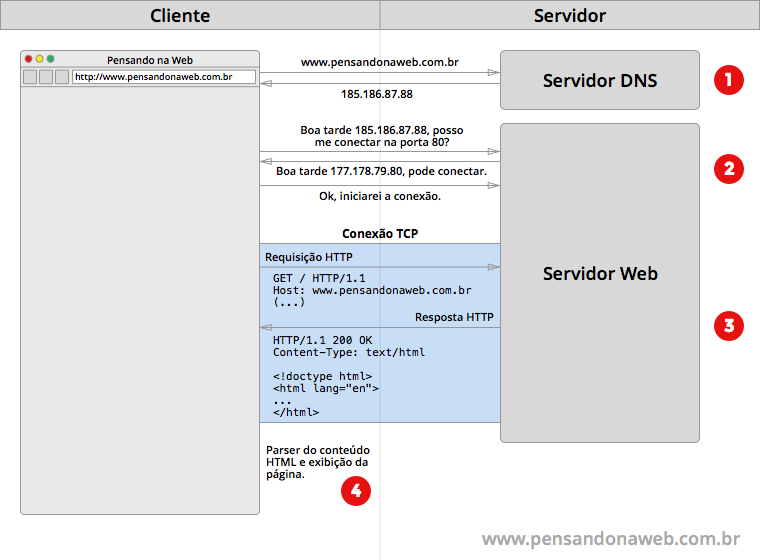
\includegraphics[width=0.7\linewidth]{dados/figuras/conexao}
    \caption{Arquitetura cliente servidor web}
    \label{fig:conexao}
\end{figure}

O HTML ou \textit{Hypertext Markup Language} é uma linguagem de marcação utilizada para criar páginas web. Ela foi criada por Tim Berners-Lee, o também criador do protocolo HTTP e da \textit{World Wide Web}, e no início suportava apenas elementos de textos e \textit{links}.

\section{HTML e CSS - Linguagens de Marcação}

Antes de falarmos em HTML5, é necessário detalhar um pouco mais o HTML. HTML significa "Linguagem de Marcação de Hipertexto". Consiste em uma linguagem de marcação utilizada para produção de páginas na web, que permite a criação de documentos que podem ser lidos em praticamente qualquer tipo de computador e transmitidos pela internet.

Para escrever documentos HTML não é necessário mais do que um editor de texto simples e conhecimento dos códigos que compõem a linguagem. Os códigos (conhecidos como \textit{tags}) servem para indicar a função de cada elemento da página \textit{Web}. Os tags funcionam como comandos de formatação de textos, formulários, links (ligações), imagens, tabelas, entre outros.

Os \textit{browsers} (navegadores) identificam as \textit{tags} e apresentam a página conforme está especificada. Um documento em HTML é um texto simples, que pode ser editado no Bloco de Notas (Windows) ou Editor de Texto (Mac) e transformado em hipertexto.

\section{HTML5}

Entre 1993 e 1995, o HTML ganhou as versões HTML+, HTML2.0 e HTML3.0, onde foram propostas diversas mudanças para enriquecer as possibilidades da linguagem. Contudo, até aqui o HTML ainda não era tratado como um padrão.

Quando o HTML4 foi lançado, o W3C alertou os desenvolvedores sobre algumas boas práticas que deveriam ser seguidas ao produzir códigos client-side. Desde este tempo, assuntos como a separação da estrutura do código com a formatação e princípios de acessibilidade foram trazidos para discussões e à atenção dos fabricantes e desenvolvedores.

Contudo, o HTML4 ainda não trazia diferencial real para a semântica do código. o HTML4 também não facilitava a manipulação dos elementos via Javascript ou CSS. Se você quisesse criar um
sistema com a possibilidade de Drag’n Drop de elementos, era necessário criar um grande script,
com bugs e que muitas vezes não funcionavam de acordo em todos os browsers.

O HTML5 é a nova versão do HTML4. Enquanto o WHATWG define as regras de marcação que usaremos no HTML5 e no XHTML, eles também definem APIs que formarão a base da arquitetura web. Essas APIs são conhecidas como DOM Level 0.

Um dos principais objetivos do HTML5 é facilitar a manipulação do elemento possibilitando o desenvolvedor a modificar as características dos objetos de forma não intrusiva e de maneira que seja transparente para o usuário final.

Ao contrário das versões anteriores, o HTML5 fornece ferramentas para a CSS e o Javascript fazerem seu trabalho da melhor maneira possível. O HTML5 permite por meio de suas APIs a manipulação das características destes elementos, de forma que o website ou a aplicação continue leve
e funcional.

O HTML5 também cria novas tags e modifica a função de outras. As versões antigas do HTML não continham um padrão universal para a criação de seções comuns e específicas como rodapé, cabeçalho, sidebar, menus e etc. Não havia um padrão de nomenclatura de IDs, Classes ou tags. Não havia um método de capturar de maneira automática as informações localizadas nos rodapés
dos websites.

O HTML5 modifica a forma de como escrevemos código e organizamos a informação na página. Seria mais semântica com menos código. Seria mais interatividade sem a necessidade de instalação de plugins e perda de performance. É a criação de código interoperável, pronto para futuros dispositivos e que facilita a reutilização da informação de diversas formas.

\section{CSS}

CSS é chamado de linguagem \textit{Cascading Style Sheet} e é usado para estilizar elementos escritos em uma linguagem de marcação como HTML. O CSS separa o conteúdo da representação visual do site. Pense  na decoração da sua página. Utilizando o CSS é possível alterar a cor do texto e do fundo, fonte e espaçamento entre parágrafos. Também pode criar tabelas, usar variações de \textit{layouts}, ajustar imagens para suas respectivas telas e assim por diante.

CSS foi desenvolvido pelo W3C (\textit{World Wide Web Consortium}) em 1996, por uma razão bem simples. O HTML não foi projetado para ter tags que ajudariam a formatar a página. Você deveria apenas escrever a marcação para o site.

\section{CSS3}

Apesar de lançada em 2010, CSS3 é a última versão da Folha de Estilo em Cascata e veio para acrescentar de forma melhorada das versões anteriores.

A melhor novidade é em relação a flexibilidade na criação de layouts, trazendo mais autonomia para os webdesigners e também desenvolvedores, que de certa forma estão ligados ao visual do site.

Com o CSS3, é possível elaborar cantos arredondados, sombras, efeitos gradientes, animações e efeitos de transição, dentre outras opções.

\section{HTML5 e CSS3}

O HTML5 foi desenvolvido para atender as crescentes demandas apresentadas pelas necessidades atuais da mídia, cross-device e internet móvel. Podemos dizer que é uma ótima ferramenta para desenvolvimento de aplicativos móveis multiplataforma porque muitos dos seus recursos foram adaptados com a consideração de acesso em dispositivos de baixa potência, incluindo Tablets e Smartphones.

Para uma adição, o HTML5 oferece uma interface comum para tornar os componentes de carregamento mais simples. Por exemplo, o HTML5 não requer o plugin Flash porque o elemento será executado sozinho.

\begin{figure}[!htb]
    \centering
    \sbox0{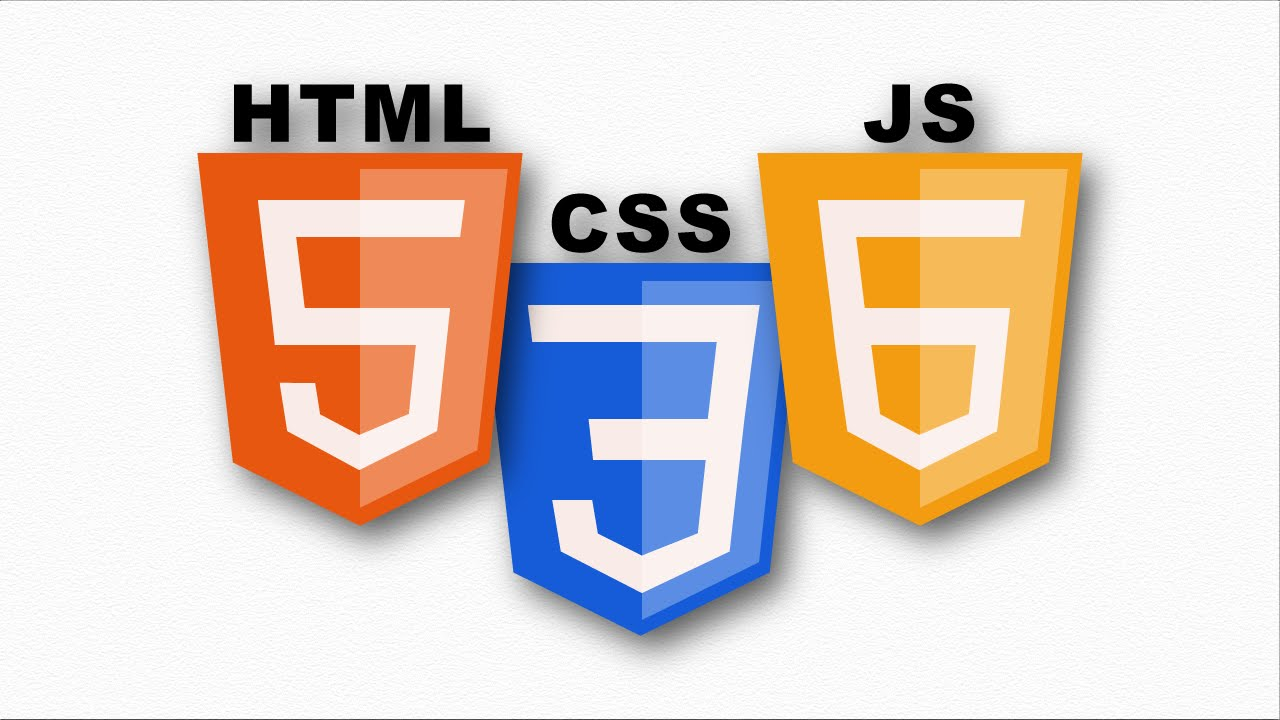
\includegraphics[width=0.5\textwidth]{./dados/figuras/figura4}}	% measure width
    \begin{minipage}{\wd0}
    \usebox0
        \caption{HTML5 CSS3 JS6 - adaptada pelo autor}
    \end{minipage}
\end{figure}

\section{Sugestão}

Com o intuito de permitir uma rápida expansão Empresa de Roupas T-Shirt, definiu-se em utilizar o HTML5 e o CSS3, que irá propor um desenvolvendo e expandindo do conteúdo na \textit{web} e aplicativos mobile, que podem acessar em diferentes dispositivos, navegadores e sistemas operacionais.

